\subsection{Tipo de entidad Pregunta Oficial}

   \begin{description}

   \item[Definición] Se refiere al objeto del mundo real: \emph{``Cuestión
   perteneciente a una plantilla de entrevista oficial planteada por el usuario
   asesor al usuario alumno''}.

   \item[Características] La entidad presenta las siguientes características:
      \begin{itemize}
         \item \textbf{Nombre:} Pregunta Oficial.
         \item \textbf{Tipo:} Débil por identificación con respecto a
         Plantilla Entrevista Oficial.
         \item \textbf{Número de atributos:} 3 propios y 1 heredado.
         \item \textbf{Atributo/s identificador/es principal/es:} id\_entrevista\_oficial
         junto con id\_pregunta\_oficial.
         \item \textbf{Atributo/s identificador/es alternativo/s:} -
         \item \textbf{Atributo/s heredado/s:} id\_entrevista\_oficial del tipo
         de entidad Plantilla Entrevista Oficial.
      \end{itemize}

   \item[Diagrama] La figura \ref{diagramaPregOfi} muestra el diagrama de la entidad.
   \item \begin{figure}[!ht]
            \begin{center}
            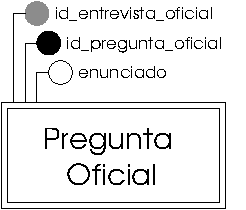
\includegraphics[]{07.Modelo_Entidad-Interrelacion/7.2.Analisis_Entidades/diagramas/preg_ofi.pdf}
            \caption{Diagrama de la entidad Pregunta Oficial.}
            \label{diagramaPregOfi}
            \end{center}
         \end{figure}

   \item[Descripción de los atributos propios] La entidad presenta los siguientes
   atributos propios:

   \begin{itemize}
    \item \textbf{id\_pregunta\_oficial}
      \begin{itemize}
         \item \textbf{Definición:} Código que sirve como número identificativo
               para cada pregunta oficial del sistema.
         \item \textbf{Dominio:} Números naturales.
         \item \textbf{Carácter:} Obligatorio.
         \item \textbf{Ejemplo práctico:} 55.
         \item \textbf{Información adicional:} El dato lo genera el sistema
               cuando se introduce una nueva pregunta oficial en el sistema. Es
               la clave primaria.
      \end{itemize}
   \item \textbf{enunciado}
      \begin{itemize}
         \item \textbf{Definición:} Cuestión perteneciente a una entrevista
         oficial, planteada a un alumno.
         \item \textbf{Dominio:} Conjunto de caracteres alfanuméricos.
         \item \textbf{Carácter:} Obligatorio.
         \item \textbf{Ejemplo práctico:} ¿Quién le ha informado de esta
         carrera?.
         \item \textbf{Información adicional:} El dato lo introduce el
         administrador principal al introducir una nueva pregunta oficial en el
         sistema.
      \end{itemize}
    \item \textbf{última\_modificación}
      \begin{itemize}
         \item \textbf{Definición:} Establece el día, mes y año cuando se
            produjo la última modificación de la entidad.
         \item \textbf{Dominio:} Formato de fecha: dd/mm/aaaa.
         \item \textbf{Carácter:} Opcional.
         \item \textbf{Ejemplo práctico:} 02/02/2009.
         \item \textbf{Información adicional:} El dato lo genera el sistema
               cuando se modifica una pregunta oficial en el sistema.
      \end{itemize}
   \end{itemize}

   \item[Ejemplo práctico]

   \item \begin{center}
            \begin{tabular}{ | l | l | }
            \hline
            \multicolumn{2}{ | c | }{\textbf{Tipo de entidad Pregunta Oficial}} \\
            \hline
            id\_entrevista\_oficial & 24 \\
            \hline
            id\_pregunta\_oficial & 55 \\
            \hline
            enunciado & ¿Quién le ha informado de esta carrera? \\
            \hline
            última\_modificación & 02/02/2009 \\
            \hline
            \end{tabular}
         \end{center}
   \end{description}
